\documentclass{article}

\usepackage{amssymb}

\usepackage{graphicx}
\usepackage{tikz}

\usetikzlibrary{shapes,calc}

\tikzstyle{edge}=[shorten <=2pt, shorten >=2pt,
                  >=stealth, line width=1.1pt]
\tikzstyle{blueE}=[shorten <=2pt, shorten >=2pt,
                   >=stealth, line width=1.5pt, blue]
\tikzstyle{blackV}=[circle, fill=black,
                    minimum size=6pt,
                    inner sep=0pt, outer sep=0pt]
\tikzstyle{blueV}=[circle, fill=blue, draw,
                   minimum size=6pt, line width=0.75pt,
                   inner sep=0pt, outer sep=0pt]
\tikzstyle{redV}=[circle, fill=red, draw,
                  minimum size=6pt, line width=0.75pt,
                  inner sep=0pt, outer sep=0pt]
\tikzstyle{redSV}=[semicircle, fill=red, minimum
                   size=3pt, inner sep=0pt, outer sep=0pt,
                   rotate=225]
\tikzstyle{blueSV}=[semicircle, fill=blue, minimum
                    size=3pt, inner sep=0pt, outer sep=0pt,
                    rotate=225]
\tikzstyle{blackSV}=[semicircle, fill=black, minimum
                    size=3pt, inner sep=0pt, outer sep=0pt,
                    rotate=225]
\tikzstyle{vertex}=[circle, draw, minimum size=6pt,
                    line width=0.75pt, inner sep=0pt,
                    outer sep=0pt]

\begin{document}
\begin{figure}[ht!]
\centering
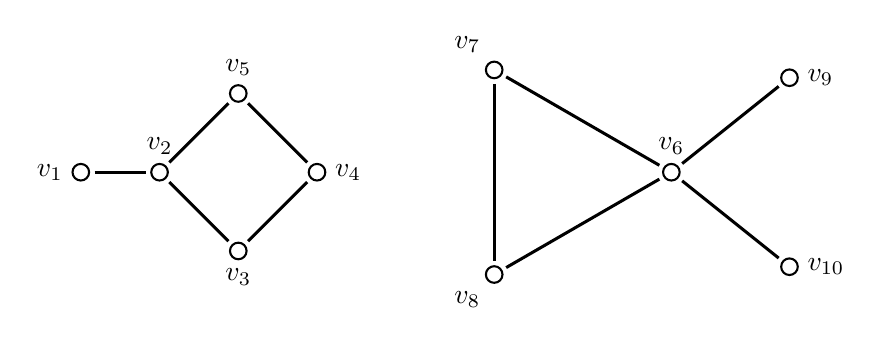
\begin{tikzpicture}
\node (0) [vertex,label=180:$v_1$] at (0,0){};
\node (1) [vertex,label=90:$v_2$]  at (1,0){};
\begin{scope}[xshift=2cm]
\node (2) [vertex,label=270:$v_3$] at (270:1){};
\node (3) [vertex,label=0:$v_4$]   at (0:1){};
\node (4) [vertex,label=90:$v_5$]  at (90:1){};
\end{scope}

\draw [edge] (0) to (1);
\draw [edge] (1) to (2);
\draw [edge] (2) to (3);
\draw [edge] (3) to (4);
\draw [edge] (4) to (1);

% Componente derecha
\begin{scope}[xshift=6cm]
\node (5) [vertex,label=90:$v_6$]     at (0:1.5){};
\node (6) [vertex,label=120:$v_7$]    at (120:1.5){};
\node (7) [vertex,label=240:$v_8$]    at (240:1.5){};
\node (8) [vertex,label=0:$v_9$]     at (3,1.2){};
\node (9) [vertex,label=0:$v_{10}$]  at (3,-1.2){};

\draw [edge] (5) to (6);
\draw [edge] (6) to (7);
\draw [edge] (7) to (5);
\draw [edge] (5) to (8);
\draw [edge] (5) to (9);
\end{scope}

\end{tikzpicture}
\caption{Una gr\'afica.}
\label{fig:grafSim}
\end{figure}






\begin{figure}[ht!]
\centering
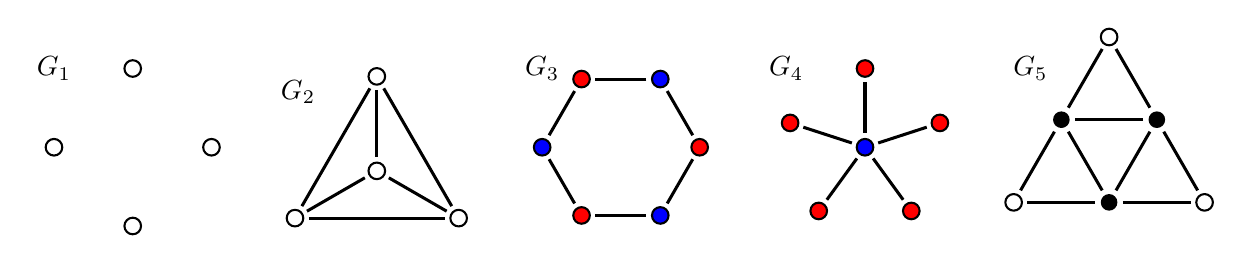
\begin{tikzpicture}
%%%%%%%%%%%%%%%%%%%%%%%%%%%%%%%%%%%%%%%%%%%%%%%%
%%%%%%%%%%         Empty Graph        %%%%%%%%%%
%%%%%%%%%%%%%%%%%%%%%%%%%%%%%%%%%%%%%%%%%%%%%%%%
\begin{scope}
% if label is needed -> label={(360/4)*\i}:$\i$
\foreach \i in {0,...,3}
	\node (\i) [vertex] at ({(360/4)*\i}:1){};

\node (L) at (-1,1){$G_1$};
\end{scope}

%%%%%%%%%%%%%%%%%%%%%%%%%%%%%%%%%%%%%%%%%%%%%%%%
%%%%%%%%%%       Complete Graph       %%%%%%%%%%
%%%%%%%%%%%%%%%%%%%%%%%%%%%%%%%%%%%%%%%%%%%%%%%%
\begin{scope}[xshift=3.1cm,yshift=-0.3cm]
\node (4) [vertex] at (0,0){};
\foreach \i in {0,1,2}
	\node (\i) [vertex] at ({90+(360/3)*\i}:1.2){};

\foreach \i in {0,1,2}
	\draw [edge] let \n1={int(mod(\i+1,3))} in (\i) to (\n1);
\foreach \i in {0,1,2}
	\draw [edge] (\i) to (4);

\node (L) at (-1,1){$G_2$};
\end{scope}


%%%%%%%%%%%%%%%%%%%%%%%%%%%%%%%%%%%%%%%%%%%%%%%%
%%%%%%%%%%       Bipartite Grap       %%%%%%%%%%
%%%%%%%%%%%%%%%%%%%%%%%%%%%%%%%%%%%%%%%%%%%%%%%%
\begin{scope}[xshift=6.2cm,yshift=0cm]
\foreach \i in {0,2,4}
	\node (\i) [redV]  at ({(360/6)*\i}:1){};
\foreach \i in {1,3,5}
	\node (\i) [blueV] at ({(360/6)*\i}:1){};


\foreach \i in {0,...,5}
	\draw [edge] let \n1={int(mod(\i+1,6))} in (\i) to (\n1);

\node (L) at (-1,1){$G_3$};
\end{scope}


%%%%%%%%%%%%%%%%%%%%%%%%%%%%%%%%%%%%%%%%%%%%%%%%
%%%%%%%%%%            Star            %%%%%%%%%%
%%%%%%%%%%%%%%%%%%%%%%%%%%%%%%%%%%%%%%%%%%%%%%%%
\begin{scope}[xshift=9.3cm]
\node (6) [blueV] at (0,0){};
\foreach \i in {0,...,4}
	\node (\i) [redV] at ({90+(360/5)*\i}:1){};

\foreach \i in {0,...,4}
	\draw [edge] (\i) to (6);

\node (L) at (-1,1){$G_4$};
\end{scope}


%%%%%%%%%%%%%%%%%%%%%%%%%%%%%%%%%%%%%%%%%%%%%%%%
%%%%%%%%%%           Split            %%%%%%%%%%
%%%%%%%%%%%%%%%%%%%%%%%%%%%%%%%%%%%%%%%%%%%%%%%%
\begin{scope}[xshift=12.4cm]
\foreach \i in {0,2,4}
	\node (\i) [blackV] at ({30+(360/6)*\i}:0.7){};
\foreach \i in {1,3,5}
	\node (\i) [vertex] at ({30+(360/6)*\i}:1.4){};

\foreach \i in {0,...,5}
	\draw [edge] let \n1={int(mod(\i+1,6))} in (\i) to (\n1);
\foreach \i in {0,2,4}
	\draw [edge] let \n1={int(mod(\i+2,6))} in (\i) to (\n1);

\node (L) at (-1,1){$G_5$};
\end{scope}


\end{tikzpicture}
\caption{Ejemplos de gr\'aficas vac\'ia, completa,
bipartita, bipartita completa y escindible.}
\label{fig:fam1}
\end{figure}





\begin{figure}[ht!]
\centering
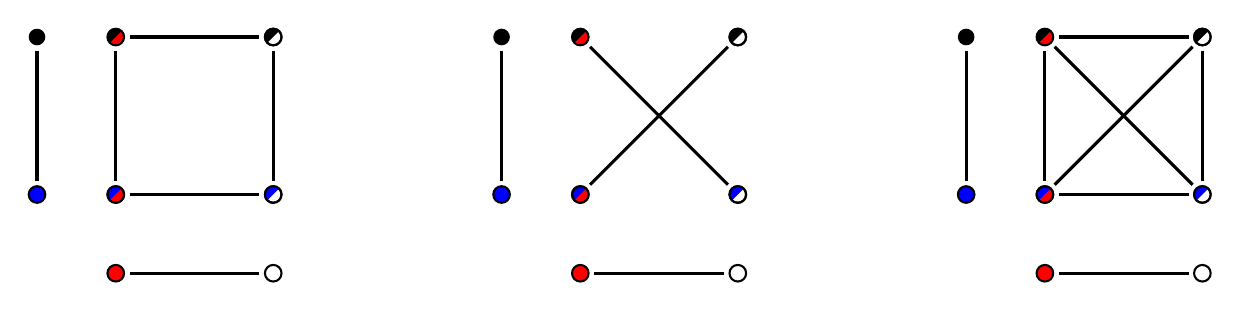
\begin{tikzpicture}
%%%%%%%%%%%%%%%%%%%%%%%%%%%%%%%%%%%%%%%%%%%%%%%%
%%%%%%%%%%          Cartesian         %%%%%%%%%%
%%%%%%%%%%%%%%%%%%%%%%%%%%%%%%%%%%%%%%%%%%%%%%%%
\begin{scope}
\node (a) [blackV] at (-2,1){};
\node (b) [blueV] at (-2,-1){};

\node (c) [vertex] at (1,-2){};
\node (d) [redV] at (-1,-2){};

\node (ad) [vertex] at (45:1.4142){};
\node      [blackSV,anchor=south,rotate=180] at (ad.center){};
\node (0)  [vertex] at (45:1.4142){};

\node (ac) [blackV] at (135:1.4142){};
\node      [redSV,anchor=south] at (ac.center){};
\node (1)  [vertex] at (135:1.4142){};

\node (bc) [blueV] at (225:1.4142){};
\node      [redSV,anchor=south] at (bc.center){};
\node (2)  [vertex] at (225:1.4142){};

\node (bd) [vertex] at (315:1.4142){};
\node      [blueSV,anchor=south,rotate=180] at (bd.center){};
\node (3)  [vertex] at (315:1.4142){};

\foreach \i in {0,...,3}
	\draw [edge] let \n1={int(mod(\i+1,4))} in (\i) to (\n1);
\foreach \i/\j in {a/b,c/d}
	\draw [edge] (\i) to (\j);
\end{scope}

%%%%%%%%%%%%%%%%%%%%%%%%%%%%%%%%%%%%%%%%%%%%%%%%
%%%%%%%%%%           Tensor           %%%%%%%%%%
%%%%%%%%%%%%%%%%%%%%%%%%%%%%%%%%%%%%%%%%%%%%%%%%
\begin{scope}[xshift=5.9cm]
\node (a) [blackV] at (-2,1){};
\node (b) [blueV] at (-2,-1){};

\node (c) [vertex] at (1,-2){};
\node (d) [redV] at (-1,-2){};

\node (ad) [vertex] at (45:1.4142){};
\node      [blackSV,anchor=south,rotate=180] at (ad.center){};
\node (0)  [vertex] at (45:1.4142){};

\node (ac) [blackV] at (135:1.4142){};
\node      [redSV,anchor=south] at (ac.center){};
\node (1)  [vertex] at (135:1.4142){};

\node (bc) [blueV] at (225:1.4142){};
\node      [redSV,anchor=south] at (bc.center){};
\node (2)  [vertex] at (225:1.4142){};

\node (bd) [vertex] at (315:1.4142){};
\node      [blueSV,anchor=south,rotate=180] at (bd.center){};
\node (3)  [vertex] at (315:1.4142){};

\foreach \i/\j in {0/2,1/3,a/b,c/d}
	\draw [edge] (\i) to (\j);
\end{scope}


%%%%%%%%%%%%%%%%%%%%%%%%%%%%%%%%%%%%%%%%%%%%%%%%
%%%%%%%%%%           Strong           %%%%%%%%%%
%%%%%%%%%%%%%%%%%%%%%%%%%%%%%%%%%%%%%%%%%%%%%%%%
\begin{scope}[xshift=11.8cm]
\node (a) [blackV] at (-2,1){};
\node (b) [blueV] at (-2,-1){};

\node (c) [vertex] at (1,-2){};
\node (d) [redV] at (-1,-2){};

\node (ad) [vertex] at (45:1.4142){};
\node      [blackSV,anchor=south,rotate=180] at (ad.center){};
\node (0)  [vertex] at (45:1.4142){};

\node (ac) [blackV] at (135:1.4142){};
\node      [redSV,anchor=south] at (ac.center){};
\node (1)  [vertex] at (135:1.4142){};

\node (bc) [blueV] at (225:1.4142){};
\node      [redSV,anchor=south] at (bc.center){};
\node (2)  [vertex] at (225:1.4142){};

\node (bd) [vertex] at (315:1.4142){};
\node      [blueSV,anchor=south,rotate=180] at (bd.center){};
\node (3)  [vertex] at (315:1.4142){};

\foreach \i in {0,...,3}
	\draw [edge] let \n1={int(mod(\i+1,4))} in (\i) to (\n1);
\foreach \i/\j in {0/2,1/3,a/b,c/d}
	\draw [edge] (\i) to (\j);
\end{scope}

\end{tikzpicture}
\caption{Las gr\'aficas $K_2 \Box K_2$, $K_2
\times K_2$ y $K_2 \boxtimes K_2$.}
\label{fig:productos}
\end{figure}





\end{document}
